\addcontentsline{toc}{chapter}{APPENDIX A - GGR 2018 PARTICIPANT GUIDE}

\setcounter{table}{0}
\renewcommand{\thetable}{A. \arabic{table}}

\setcounter{figure}{0}
\renewcommand{\thefigure}{A. \arabic{figure}}

\setcounter{section}{0}
\renewcommand{\thesection}{A.\arabic{section}}

\chapter*{APPENDIX A\\GGR 2018 PARTICIPANT GUIDE}

\section{Welcome to the 2018 Great Gr\'evy's Rally}

\noindent On the 27th and 28th of January 2018, you will be part of a historic event that will take place in northern Kenya. Within 45 censusing blocks spread across the country, scientists, local community members, and citizens will drive, fly, and take photographs. The area that you will help to cover consists of the core range for the Gr\'evy's zebra and reticulated giraffe, which are the two target species of the Rally.  Only in Kenya has such an extensive census by the public, covering over 25,000 KM2, ever been completed.

Our team pioneered such a massive effort during the first Great Gr\'evy's Rally in 2016, when it was estimated that 2,350 Gr\'evy's zebra roamed the semi-arid regions of Kenya.  This year we are expanding the Rally to 1) include more participants and 2) add the reticulated giraffe, a species the IUCN has recently listed as threatened.  The tens  - or hundreds - of thousands of pictures that you will help to collect over the next two days will be uploaded to Wildbook and given to image analysis algorithms.  Our algorithms work to identify each unique animal by performing a ``sight-resight'' analysis, a non-invasive variant of the traditional ``mark-recapture'' techniques used by population biologists.  Using the visual appearance of Gr\'evy's zebras with their naturally barcoded stripes and the distinctive polygon patterns on reticulated giraffes, scientists will be able to estimate the size of animal populations within each county and across the entire nation.  We will also use your pictures to determine the age and sex of the animals so that we can estimate the health and sustainability of the population.  By being a volunteer for the Rally, your contributions will go directly towards protecting these animals and ensuring the future of their species.

For the Great Gr\'evy's Rally to succeed in 2018, it is essential that each participant follow some simple rules and guidelines.  This document will introduce you to your GGR camera (and camera supplies) and provide examples of pictures to take.

\section{Hardware Tote Bag}

\noindent Your tote bag contains the following:

\begin{itemize}
    \item A \textbf{plastic camera bag with}:
          \begin{itemize}
              \item A Nikon COOLPIX S9900 digital camera, with a carrying case
              \item USB charging cable and base charger
              \item A Kenyan plug adaptor OR USB car charger
              \item A CAMERA ID CARD (with the GGR logo, QR code, a number and letter).
          \end{itemize}
\end{itemize}

\noindent \textit{The CAMERA ID CARDS are used to organize all of the different cameras and their images during the Rally.  You will be asked to take a photograph of your CAMERA ID CARD at the beginning of each day, synchronized with all other cameras in your vehicle (if any), so please make sure it is not misplaced.}

\begin{itemize}
    \item This \textbf{participant guide packet}, which includes:
          \begin{itemize}
              \item \textbf{Introduction to your GGR Camera}
              \item \textbf{Use of Personal Digital Cameras}
              \item \textbf{Rally Day Start}  -  \textit{the procedure to follow at the start of each day}
              \item \textbf{Turning on Your GGR Camera's GPS Function}
              \item \textbf{Examples of Good and Bad Pictures}  -  \textit{a green/red reference sheet}
          \end{itemize}
\end{itemize}

\section{Introduction to Your Camera}

Each vehicle has been assigned a single, numbered GGR camera with built-in GPS.

\textbf{DO NOT remove the camera battery.} The time and date settings have been set on the camera to Kenyan time.  If the battery is removed, then the camera will revert to default settings.  If the time and date need to be reset, refer to page 13 of the camera manual.

The D-Pad is the circle directly above the MENU button with four icons and an OK button in the center.

To prepare for your first day of the Rally, take the following steps:
\begin{enumerate}
    \item Make sure the satellite icon is visible on the bottom left of the display (above the battery icon), which indicates that the GPS function has been turned on. A red satellite icon means that the camera has not found sufficient GPS satellites to function correctly. Take the camera outside with a clear view of the sky and wait 5 minutes to acquire the GPS signals.
    \item When the camera is fully connected, white boxes will appear next to the satellite icon. See the guidelines below:
\end{enumerate}

\begin{figure}[H]
    \begin{center}
        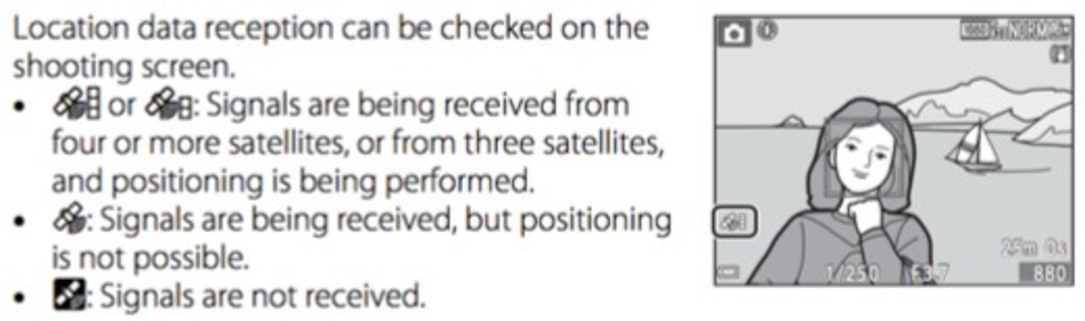
\includegraphics[width=0.8\linewidth]{resources/guide1.pdf}
    \end{center}
    \caption{GGR-18 participant guide, image 1.}
\end{figure}

\begin{center}
    \textbf{If there is NO satellite icon on the display, follow the below instructions for} \textbf{Turning on Your GGR Camera's GPS Function}
\end{center}

\section{Use of Personal Digital Cameras During the Rally}

If you are a passenger in a GGR vehicle and want to use a personal digital camera, please follow the instructions below.  Once these steps are complete, you can continue with the \textbf{Rally Day Start} procedure just like other GGR cameras.

\begin{enumerate}
    \item Ensure your camera is fully charged and bring extra batteries, if possible.
    \item Set the time and date to Kenyan time (GMT+3)
    \item Shoot in JPEG mode only (no RAW).  Pictures from film cameras can not be used.
    \item If your camera has a Digital Zoom function, turn it off or only use optical zoom
    \item Obtain a CAMERA ID CARD with the letter B, C, D, E, or F from your GGR driver.  Be sure to take a photo of your card at exactly the same time as your driver takes a picture of their card.  These simultaneous pictures will sync your pictures with the GPS records that the driver's GGR camera will create.
\end{enumerate}

\section{Rally Day Start}

\textit{Start Here Each Morning of the Rally}

\subsection{Start of the Day's Rally - Start GPS Log}

\begin{enumerate}
    \item \textit{If you are using a personal camera, continue to Step (2) on next page.}
    \item Press the MENU button to open the camera menu
    \item Push left on the D-Pad to select a menu page
    \item Push down on the D-Pad 3 times to highlight the GPS satellite icon
    \item Push the OK button
    \item Push down on the D-Pad 3 times to highlight \textbf{Create Log}
    \item Push the OK button.  Your screen should look like this:

          \begin{figure}[H]
              \begin{center}
                  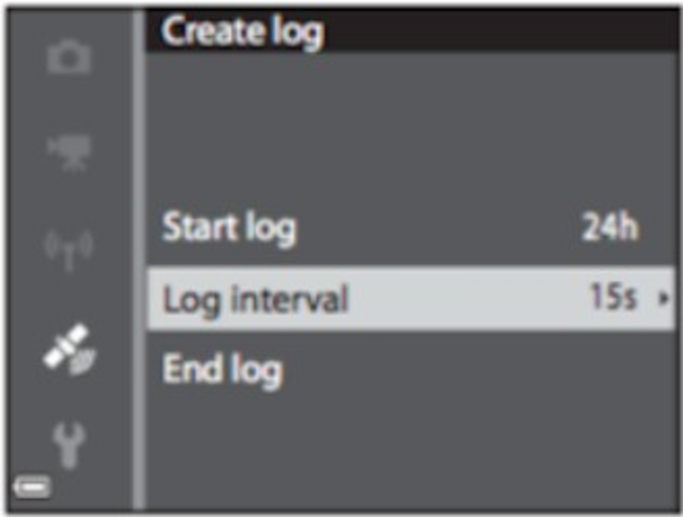
\includegraphics[width=0.4\linewidth]{resources/guide3.pdf}
              \end{center}
              \caption{GGR-18 participant guide, image 2.}
          \end{figure}

    \item If the \textbf{Log Interval} is already set to 10s, skip to step 12.
    \item Push down on the D-Pad 1 time to highlight \textbf{Log Interval}
    \item Push the OK button. Your screen should look like this:

          \begin{figure}[H]
              \begin{center}
                  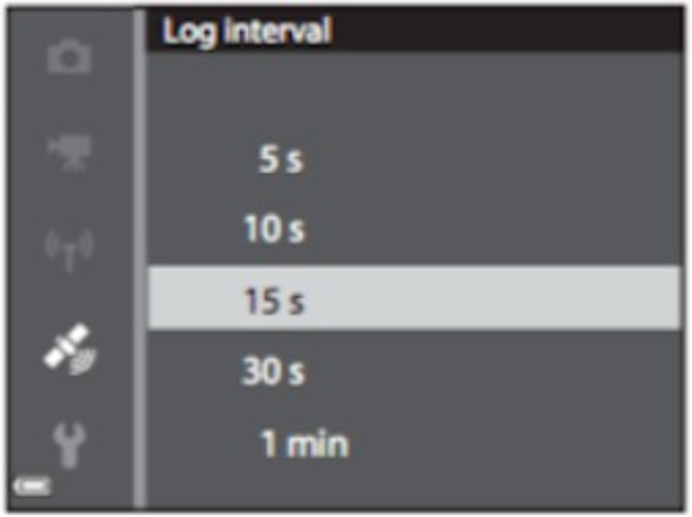
\includegraphics[width=0.4\linewidth]{resources/guide2.pdf}
              \end{center}
              \caption{GGR-18 participant guide, image 3.}
          \end{figure}

    \item Push up on the D-Pad 1 time to highlight \textbf{10s}
    \item Push the OK button
    \item Push up on the D-Pad 1 time to highlight \textbf{Start Log}
    \item Push the OK button
    \item Push down on the D-Pad 1 time to highlight \textbf{Log data for next 12 hrs}
    \item Push the OK button
    \item Your screen should look like this:

          \begin{figure}[H]
              \begin{center}
                  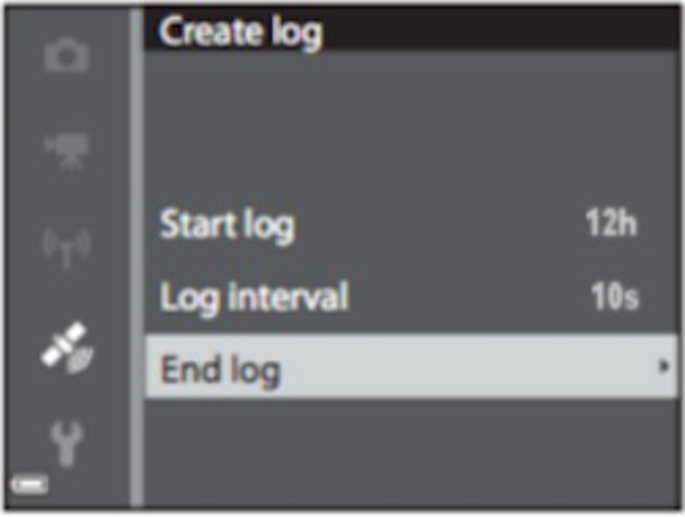
\includegraphics[width=0.4\linewidth]{resources/guide5.pdf}
              \end{center}
              \caption{GGR-18 participant guide, image 4.}
          \end{figure}

    \item \textit{Now your tracking log has started!}
    \item Verify that the highlighted menu item at the bottom says \textbf{End log} and that the duration and interval numbers are correct
          \begin{enumerate}
              \item \textbf{NOTE: DO NOT} select \textbf{End log} (this is done at the end of the day)
          \end{enumerate}
    \item Press the MENU button to close the camera menu
    \item The satellite icon on the bottom left of display (above the battery icon) should display the word \textbf{LOG} to indicate that GPS logging is turned on
\end{enumerate}

\subsection{Take a Synchronized Picture of All Camera ID Cards}

\begin{enumerate}
    \item At the same time, all cameras in the vehicle will take a single, synchronized picture of their assigned CAMERA ID CARD.  Each camera should take a picture of their assigned card at the start of every day.
    \item Begin a countdown for this picture by having the driver say, out loud, ``3-2-1 SNAP!''.  A reminder to take this picture is shown at the bottom of the card.
    \item The GGR camera should always have a CAMERA ID CARD with the letter A

          \begin{figure}[H]
              \begin{center}
                  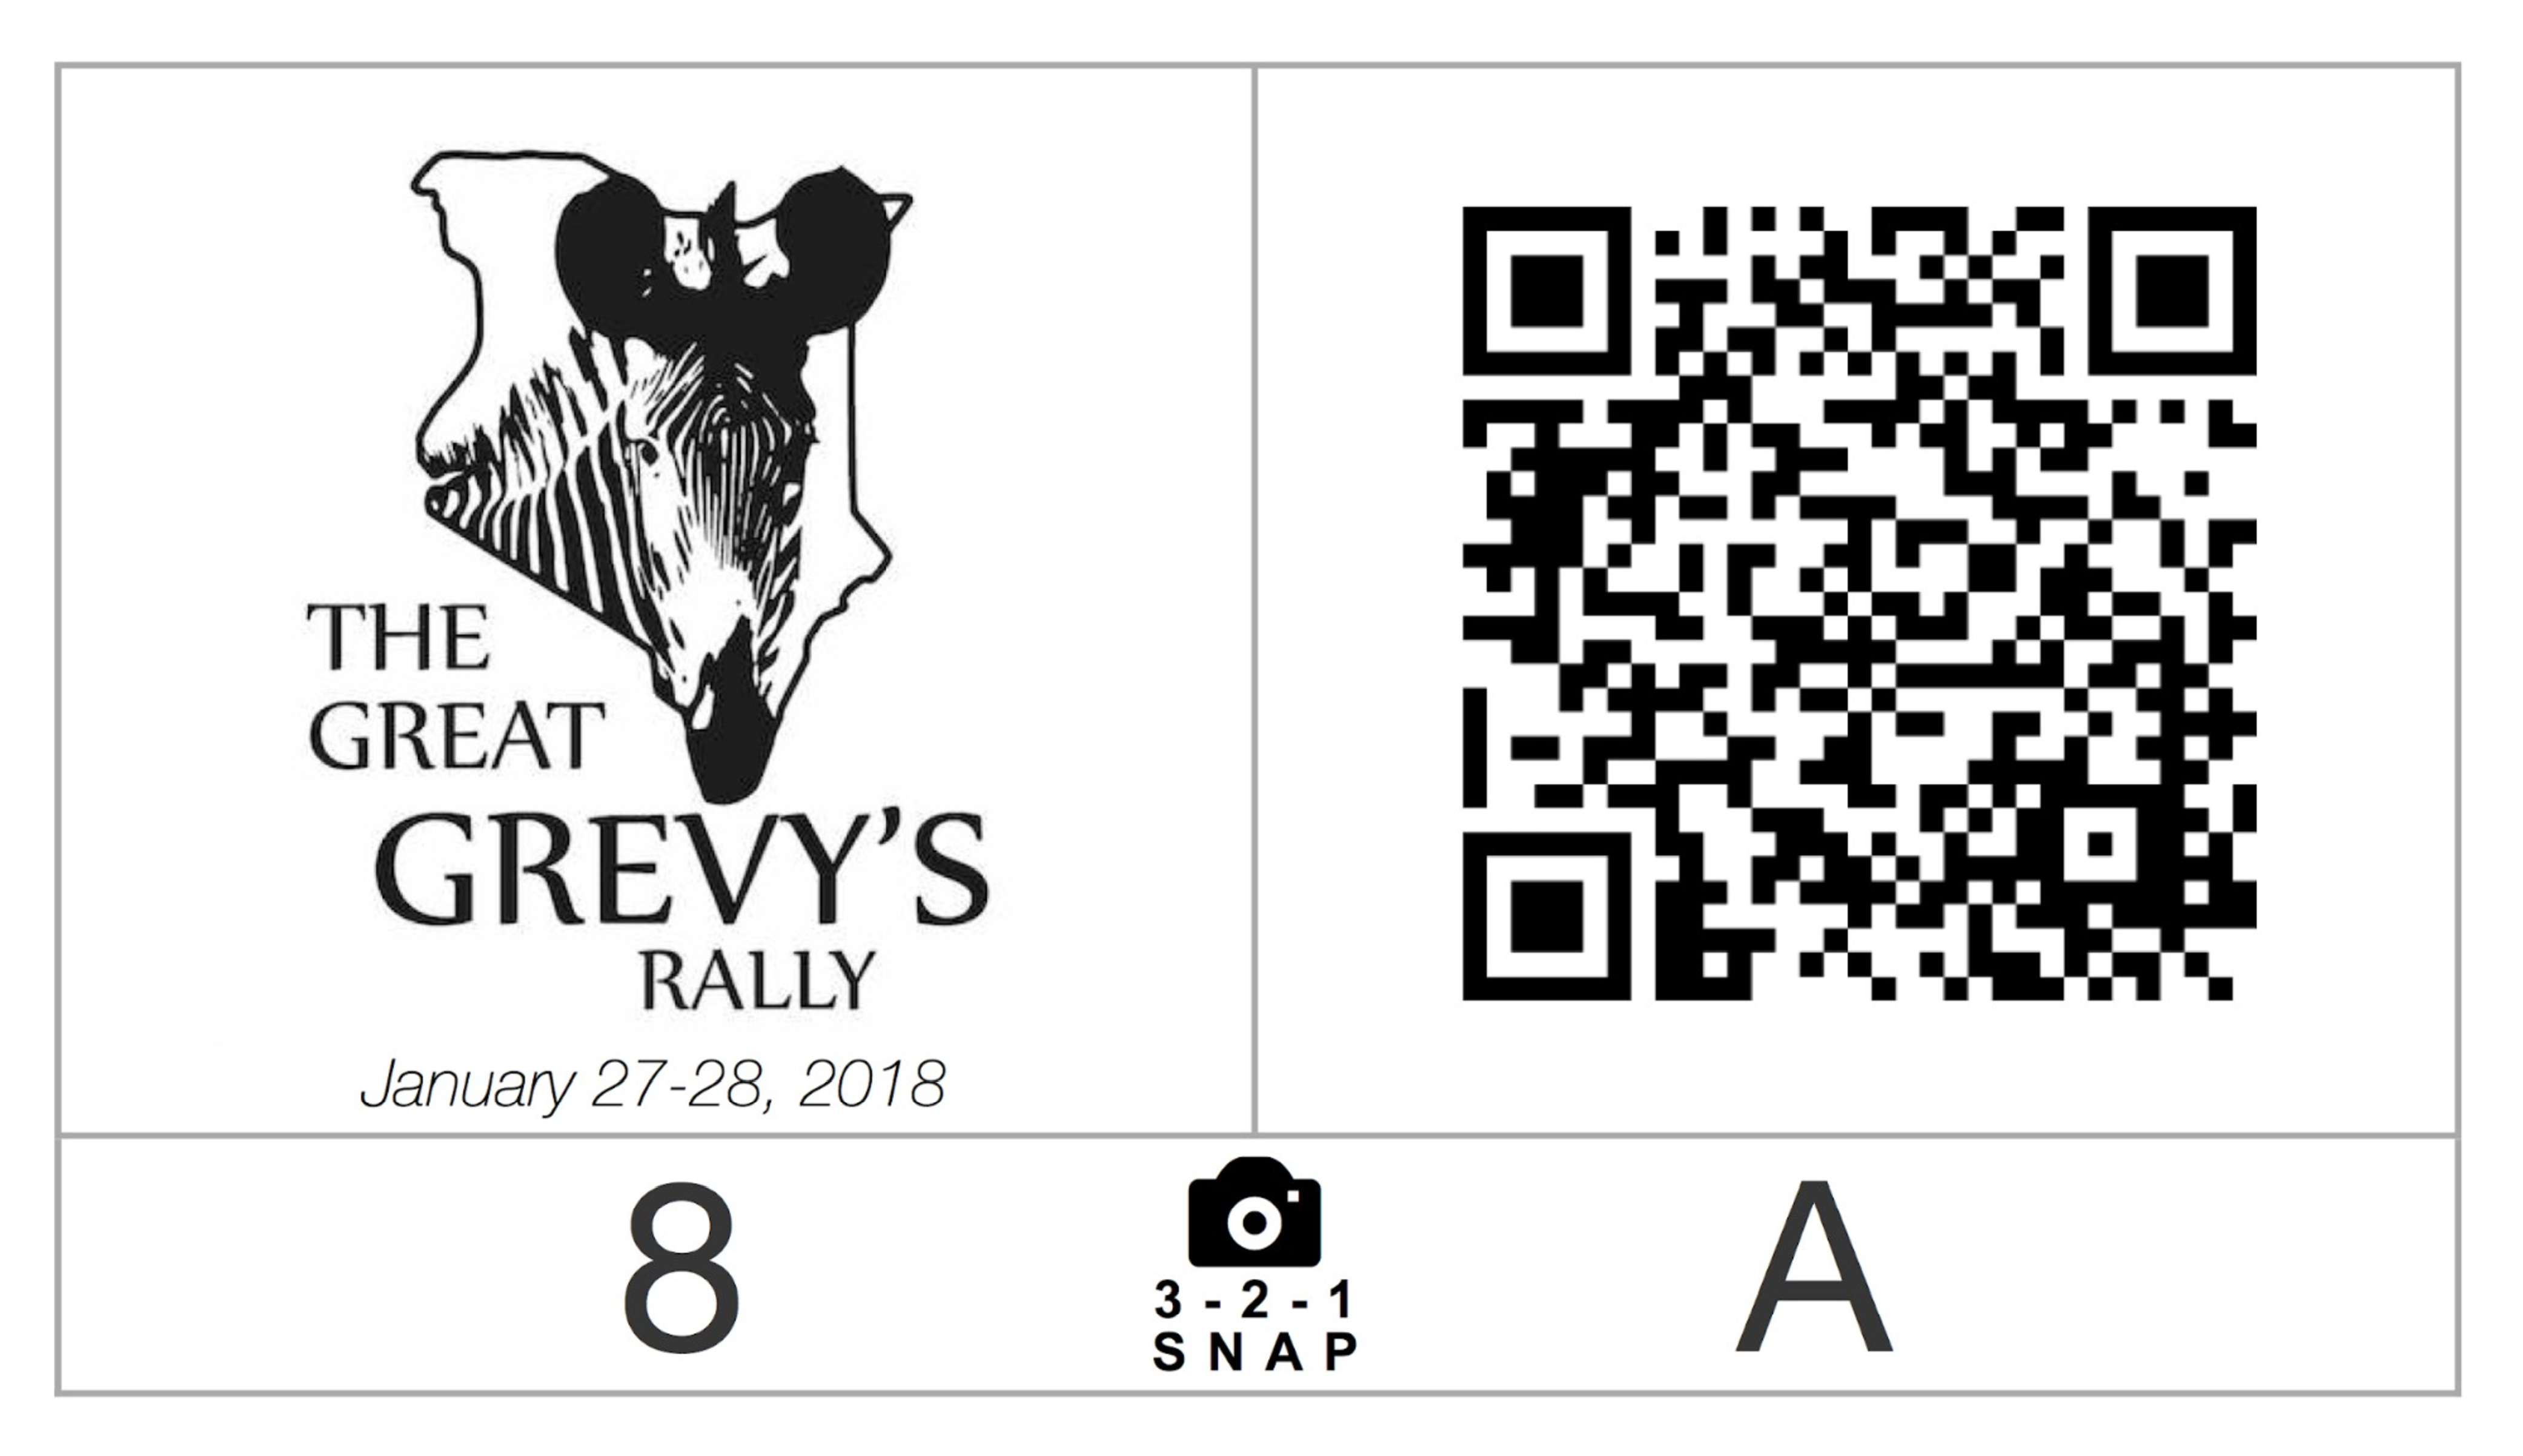
\includegraphics[width=0.8\linewidth]{resources/guide4.pdf}
              \end{center}
              \caption{GGR-18 participant guide, image 5.}
          \end{figure}

    \item If there is more than one photographer in a vehicle, each camera is assigned a CAMERA ID CARD.  All additional cameras should use the letters B, C, D, E, or F, with A being reserved for the (only or primary) GGR camera in the car.
    \item Save your CAMERA ID CARD for it is needed at the start of each day of the Rally.
\end{enumerate}

\subsection{Start your Rally!}
Go drive (or fly) to find Gr\'evy's zebras and reticulated giraffes in the wild!

\subsection{Taking Pictures of Gr\'evy's Zebras and Reticulated Giraffes}

\begin{enumerate}
    \item Photographing the animals
          \begin{enumerate}
              \item \textbf{Group Photos} - As you approach, take a photo of the Gr\'evy's zebra herd or the tower of giraffes from a distance.  Try to capture the entire herd using only 1 or 2 images. Do this even if a single Gr\'evy's zebra or reticulated giraffe is seen alone.
              \item \textbf{Individual Photos} - After you have taken the group photo from a distance, approach the group of animals to get a closer look and take photos of each individual animal.
          \end{enumerate}
    \item \textbf{Target one animal at a time.  Take a picture of only the RIGHT side of the animal (facing or walking to the right).}  To ensure the best possible chance of identifying the animal, try to put the animal in the \textbf{CENTER} of the image and try to photograph the entire animal (not just a piece of it).  Refer to the green/red reference sheet for good and bad examples.
    \item Repeat Step 2 for each Gr\'evy's zebra or reticulated giraffe seen in the group.  You should aim to take 3-4 different RIGHT side pictures of each zebra or giraffe as it moves around.  Don't worry if an animal moves away or behind something (bushes or other animals) while taking photographs – the most important thing is to get at least one RIGHT side photograph for each animal in the group.
    \item \textit{Be patient!}  The animals will be curious about you and will move around slowly.  Try to wait for when you can clearly see the RIGHT side of the animal without harsh sunlight glare.  Avoid taking pictures of animals that are significantly behind bushes or other animals.  You may need to relocate yourself to find a better spot to get good, RIGHT side photos of individuals.
    \item If after a while you cannot get any pictures of the RIGHT side or if the animals start to run off, then take any picture possible.
\end{enumerate}

\newpage

\begin{center}
    \textit{
        \large{
            Remember: ``Right is Right!''
        }
    }
\end{center}

\begin{center}
    \textit{
        \large{
            Only take pictures of the RIGHT side of a zebra or giraffe.
        }
    }
\end{center}

\subsection{End of the Day's Rally - End GPS Log}

\begin{enumerate}
    \item \textbf{If you are using a personal camera, continue to Step (6) at the bottom of page}
    \item Press the MENU button to open the camera menu
    \item Push left on the D-Pad to select a menu page
    \item Push down on the D-Pad 3 times to highlight the GPS satellite icon
    \item Push the OK button
    \item Push the OK button to highlight menu item \textbf{Create log}
    \item Push the OK button
    \item Your screen should look like the image below. Push the OK button on the (already) highlighted menu item End log.

          \begin{figure}[H]
              \begin{center}
                  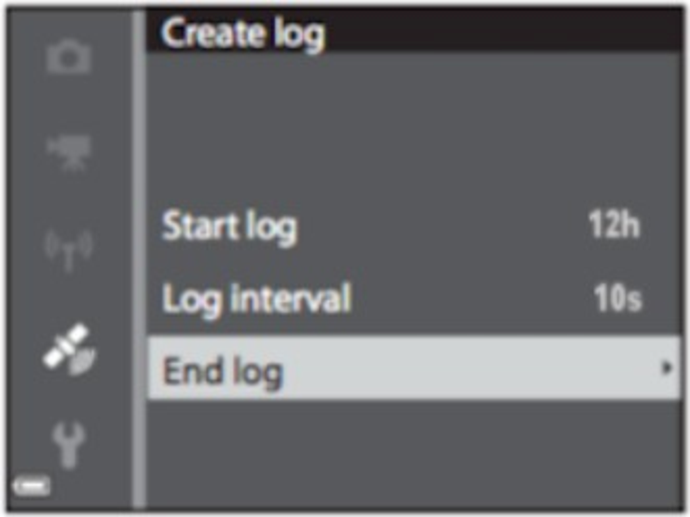
\includegraphics[width=0.4\linewidth]{resources/guide7.pdf}
              \end{center}
              \caption{GGR-18 participant guide, image 6.}
          \end{figure}

    \item Your screen should look like the image below. Push the OK button on the (already) highlighted menu item \textbf{Save log}

          \begin{figure}[H]
              \begin{center}
                  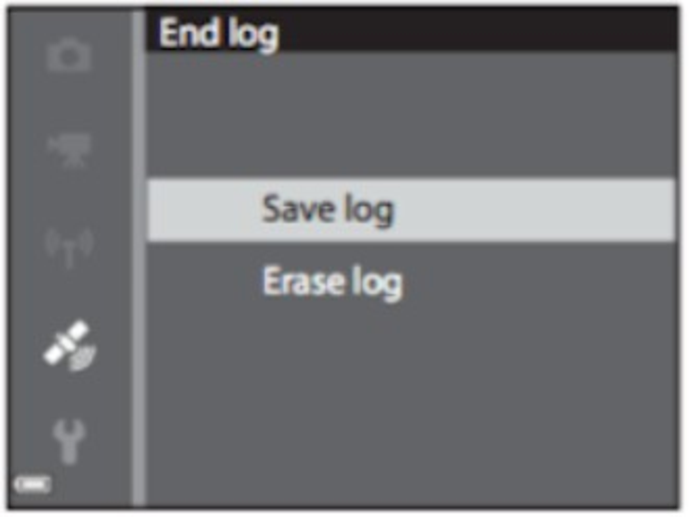
\includegraphics[width=0.4\linewidth]{resources/guide6.pdf}
              \end{center}
              \caption{GGR-18 participant guide, image 7.}
          \end{figure}

    \item This operation could take a few minutes to complete, \textbf{DO NOT} turn off the camera during this process. The screen may or may not change while it is saving the location log to the SD card. Once it is complete, a message will appear across the screen saying the log has been saved.
    \item Push the OK button
    \item Press the MENU button again to close the camera menu
\end{enumerate}

\subsection{Prepare for Day 2 of the Rally}

\begin{enumerate}
    \item Turn off your camera
    \item Charge your camera batteries overnight
    \item Save your CAMERA ID CARD.  You will need to take a synchronization picture of your card at the start of the second day of the Rally.
\end{enumerate}

\section{Turning on Your GGR Camera's GPS Function}

\begin{enumerate}
    \item Press the MENU button on the bottom right of the back of the camera (next to the display) to open the camera menu
    \item Push left on the D-Pad to select a menu page
    \item Push down on the D-Pad 3 times to highlight the GPS satellite icon
    \item Push the OK button (located in the center of the D-Pad)
    \item Push the OK button on the (already) highlighted men item \textbf{Location data options}
    \item Push the OK button on the (already) highlighted menu item \textbf{Record location data...OFF}
    \item Push up on the D-Pad to highlight On next to the satellite icon, as seen in the screen below:

          \begin{figure}[H]
              \begin{center}
                  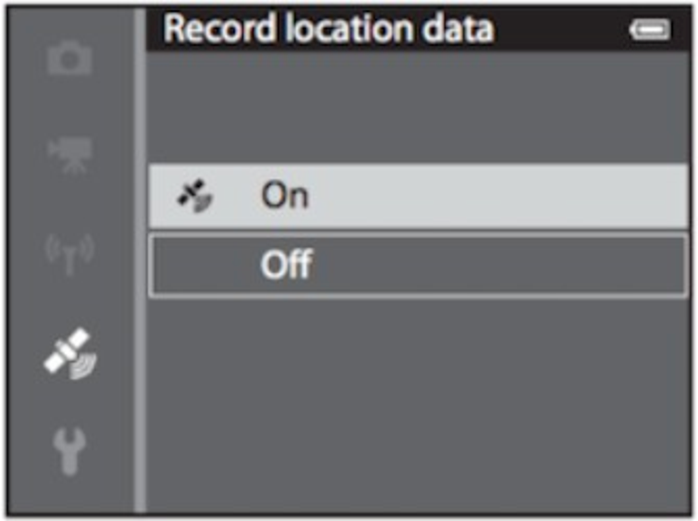
\includegraphics[width=0.4\linewidth]{resources/guide8.pdf}
              \end{center}
              \caption{GGR-18 participant guide, image 8.}
          \end{figure}

    \item Push the OK button
    \item Verify that the menu item says Record location data…ON
    \item Press the MENU button again to close the camera menu
    \item A satellite icon should appear on the bottom left of the display (above the battery icon), which indicates that the GPS function has been turned on. A red satellite icon means that the camera has not found sufficient GPS satellites to function correctly. Take the camera outside with a clear view of the sky and wait 5 minutes to acquire the GPS signals.
    \item Once the camera is fully connected, white boxes will load next to the satellite icon. See the guidelines below:
\end{enumerate}

\begin{figure}[H]
    \begin{center}
        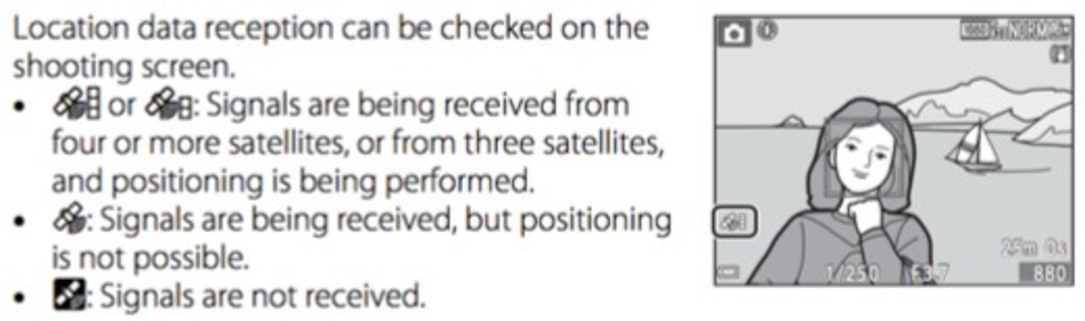
\includegraphics[width=0.8\linewidth]{resources/guide1.pdf}
    \end{center}
    \caption{GGR-18 participant guide, image 9.}
\end{figure}
